\section{Introduction}

\begin{figure}[!t!h!b!]
\centering
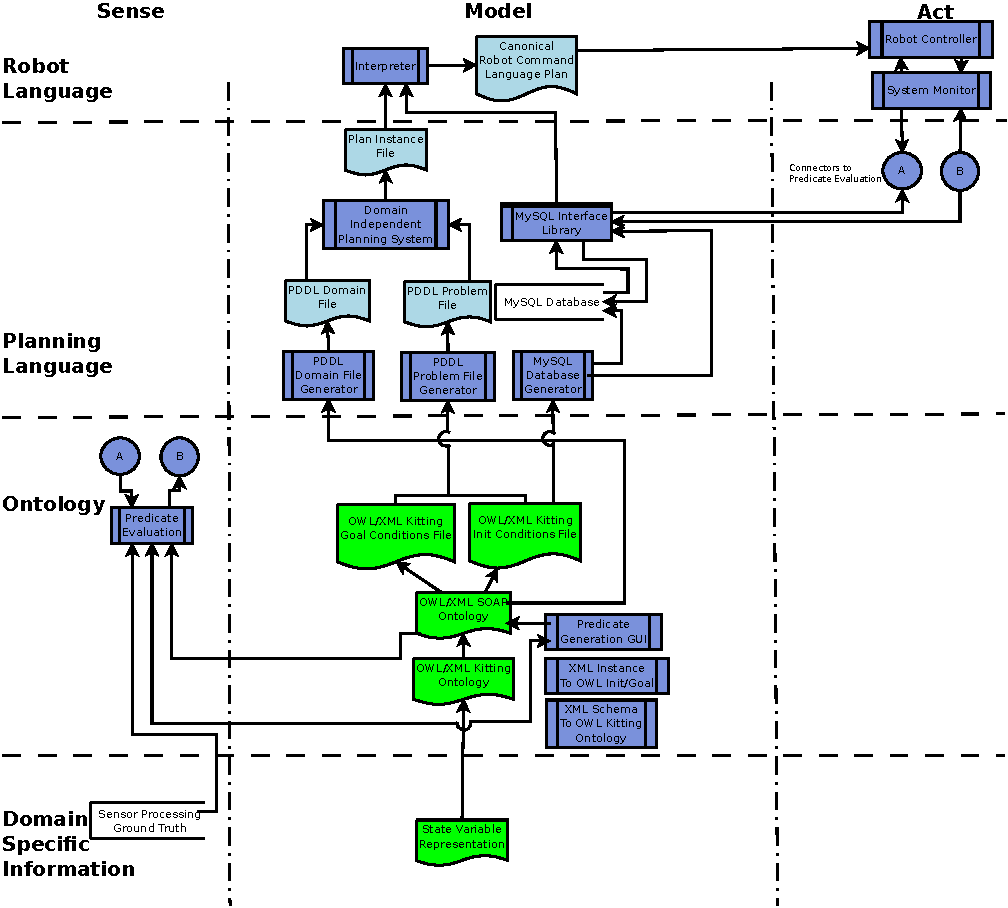
\includegraphics[width=10cm]{Figure/KnowledgeDrivenRobotics.pdf}
\caption{Knowledge Driven Design extensions -- In this figure, green shaded
  boxes with curved bottoms represent hand generated files while light blue
  shaded boxes with curved bottoms represent automatically created boxes.
  Rectangular boxes represent processes and libraries. }
\label{fig:methodology}
\end{figure}
The knowledge driven methodology presented in this section is not purposed
to act as a stand-alone system architecture. Rather it is intended to be an
extension to well developed hierarchical, deliberative architectures such
as 4D/RCS~\cite{Albus2000}. The overall knowledge driven methodology of the
system is depicted in Figure~\ref{fig:methodology}. The figure is organized
vertically by the representation that is used for the knowledge and
horizontally by the classical sense-model-act paradigm of intelligent
systems. The remainder of this section gives a brief description of each
level of the hierarchy to help the reader understand the basic concepts
implemented within the system architecture. The reader may find a more
detailed description of each component and each level of the architecture
in other documented
publications~\cite{NISTIR.Balakirsky,BALAKIRSKY.IROS.2012}.
\begin{itemize}
\item On the vertical axis, knowledge begins with Domain Specific Information
(DSI) that captures operational knowledge that is necessary to be
successful in the particular domain in which the system is designed to
operate. This includes information on items ranging from what actions and
attributes are relevant, to what the necessary conditions are for an action
to occur and what the likely results of the action are. The authors have
chosen to encode this basic information in a formalism known as a state
variable representation~\cite{NAU.2004}.

\item At the next level up, the information encoded in the DSI is then organized into a domain
independent representation. A base ontology (\textsf{OWL/XML Kitting})
contains all of the basic information that was determined to be needed
during the evaluation of the use cases and scenarios. The knowledge is
represented in as compact a form as possible with knowledge classes
inheriting common attributes from parent classes. The \textsf{OWL/XML SOAP}
ontology describes not only aspects of actions and predicates but also the
individual actions and predicates that are necessary for the domain under
study. The instance files describe the initial and goal states for the
system through the \textsf{Kitting Init Conditions File} and the
\textsf{Kitting Goal Conditions File}, respectively. The initial state file
must contain a description of the environment that is complete enough for a
planning system to be able to create a valid sequence of actions that will
achieve the given goal state. The goal state file only needs to contain
information that is relevant to the end goal of the system.
%For the case of building a kit, this may simply be that a complete kit is located in a bin designed to hold completed kits.

Since both the OWL and XML implementations of the knowledge representation are file based, real time information proved to be problematic. In order to solve this problem, an automatically generated MySQL database has been introduced as part of the knowledge representation.

\item At the next level up, aspects of this knowledge are automatically extracted and encoded in a form
that is optimized for a planning system to utilize (the Planning Language).
The planning language used in the knowledge driven system is expressed with
the Planning Domain Definition Language (PDDL)~\cite{PDDL} (version 3.0).
The PDDL input format consists of two files that specify the domain and the
problem. As shown in Figure~\ref{fig:methodology}, these files are
automatically generated from the ontology. The domain file represents
actions along with required preconditions and expected results. The problem
file represents the initial state of the system and the desired goal. From
these two files, a domain independent planning
system~\cite{Coles.ICAPS.2010} was used to produce a static \textsf{Plan Instance File}.

\item Once a plan has been formulated, the knowledge is transformed into a
representation that is optimized for use by a robotic system (the Robot
Language). The interpreter combines knowledge from the plan with knowledge
from the MySQL database to form a sequence of sequential actions that the
robot controller is able to execute. The authors devised a canonical robot
command language (CRCL) in which such lists can be written. The purpose of
the CRCL is to provide generic commands that implement the functionality of
typical industrial robots without being specific either to the language of
the planning system that makes a plan or to the language used by a robot
controller that executes a plan.
\end{itemize}

This document describes each level of the architecture from the Domain Specific Information level to the Robot Language level. The goal of this document is to help a user understand the different tools and techniques to generate the appropriate files in order to build a kit.

Each of the following section corresponds to each level of the architecture described in Figure~\ref{fig:methodology} starting from the bottom level to the top level of the architecture. 